\documentclass[a4paper]{article}

\usepackage[utf8x]{inputenc}
\usepackage{latexsym}
\usepackage[danish]{babel}
\usepackage{graphicx}
\usepackage{hyperref}
\usepackage[all]{hypcap}

\begin{document}
\title{En superkort introduktion til Emacs}

\author{Torben Mogensen}
\date{\today}

\maketitle

\begin{abstract}
I kurset ``Programmering og problemløsning'' (PoP) bruger vi
værktøjerne Emacs og \LaTeX.

Emacs er et tekstredigeringsværktøj, der er egnet til at redigere
programmer og lignende.  Ulig f.eks.\ Microsoft Word og Libre Office
Writer redigerer man ``ren'' tekst i Emacs: Der er ikke formattering
såsom fed skrift, kursiv, osv.  Til dette bruger vi \LaTeX.

Dette dokument giver en kort introduktion til Emacs.  \LaTeX{} bliver
beskrevet i et andet dokument.
\end{abstract}

\tableofcontents


\section{Emacs}

Emacs er et gratis, open-source redigeringsværktøj, der findes til
Windows, Linux, MacOS og flere andre platforme.  Emacs kan hentes fra
\url{http://www.gnu.org/software/emacs/}, hvor der også ligger
detaljeret dokumentation.  Den seneste udgave er Emacs 24.5.

\subsection{Installering af Emacs}

Her er en ultrakort vejledning til installering af Emacs på de tre
hoveplatforme.

\paragraph{Linux.}

Langt de fleste Linuxdistributioner har Emacs som en del af
standardpakkesystemet, og man kan installere det via sit
softwarecenter eller package manager.  Mange distributioner har Emacs
præinstalleret.

For at få den danske ordbog til Emacs, kan man på Debian og Ubuntu
Linux køre kommandoen \texttt{sudo~apt-get~install~aspell-da}.

\paragraph{MacOS X.} 

OS X kommer med en ældre udgave af Emacs præinstalleret, så vi
foreslår Aquamacs, som kan hentes på \url{aquamacs.org}.


For at kunne lave stavekontrol, skal du også installere
\texttt{ASpell} og den danske ordbog.  Du kan finde links til disse på
\url{http://www.latex.dtu.dk/da/page/downloads/mac}.

\paragraph{Windows.}

Gå til \url{http://ftp.gnu.org/pub/gnu/emacs/windows/} og hent
filen \texttt{emacs-24.5-bin-i686-mingw32.zip}.  Udpak denne fil i en
ny folder (kald den f.eks. \texttt{Emacs}).  Kør derefter programmet
\texttt{addpm.exe}, hvilket vil tilføje en ikon i startmenuen under
``Start → Programs → Gnu Emacs''.  Du kan evt.\ også trække filen
\texttt{runemacs.exe} til din desktop for at oprette en genvej.

For at kunne lave stavekontrol, skal du også installere
\texttt{ASpell} og den danske ordbog.  Se
\url{http://aspell.net/win32/} for en vejledning til dette. 

\section{Start og brug af emacs}

Du kan åbne Emacs ved at klikke på Emacs-ikonen (hvis du har oprettet
en sådan) eller ved at vælge en fil og åbne den med Emacs (brug
højreklick og vælg Emacs).  Du kan med fordel binde filtyperne
\texttt{.tex}, \texttt{.fs}, \texttt{.fsx} og \texttt{.fsi} til at
åbne med Emacs, da det er de filtyper, vi vil bruge Emacs til på PoP.

Du kan også på en kommandolinje skrive \texttt{emacs} efterfulgt af
navnet på den fil, du vil redigere eller oprette.  Første gang, du starter
Emacs uden at have valgt en fil, vil du se et skærmbillede i stil med

\begin{center}
%\scalebox{0.23}
{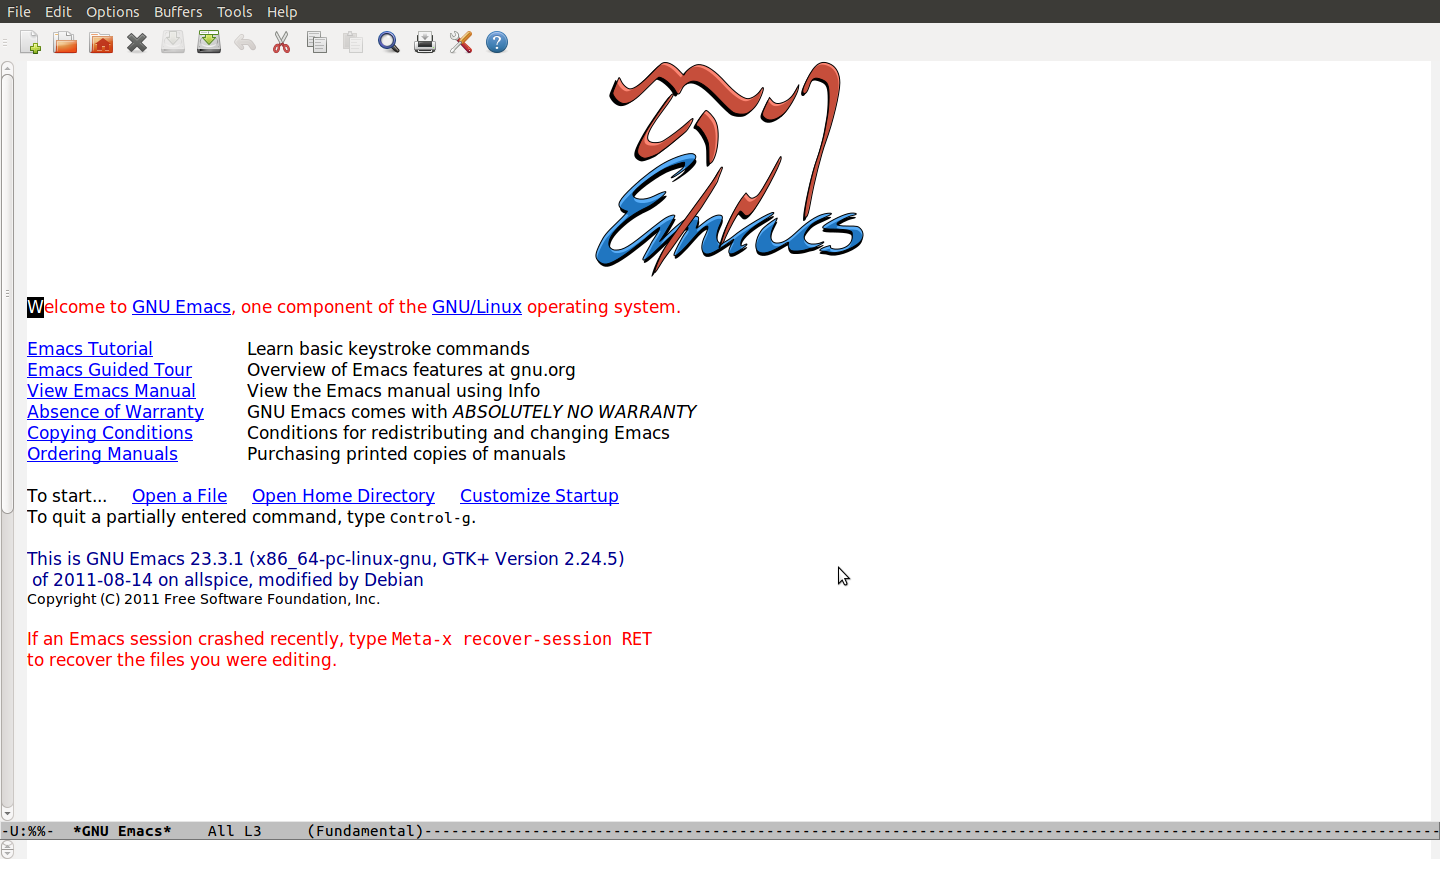
\includegraphics[width=\textwidth]{emacs-welcome.png}}
\end{center}

\noindent
Udseendet varierer lidt efter operativsystem og Emacs-version.

Du kan bruge \textsf{File} menuen til at åbne, gemme og printe filer,
lukke Emacs og flere ting -- ligesom du er vant til med
\textsf{File}-menuer.  Tilsvarende er der en \texttt{Edit}-menu med de
sædvanlige kommandoer til at klippe og klistre tekst, til at søge i
filen og flere ting.  De andre menuer gemmer vi til senere.  Under
menuerne er der ikoner til de mest almindelige opgaver såsom at hente
og gemme filer, omgøre ændringer, klippe og klistre, printe osv.  Hvis
du lader musen svæve over et ikon, kommer der en kort forklaring på funktionen.

Den største del af vinduet er \emph{bufferen}, der viser den tekst,
man er ved at redigere.  Du kan bruge mus og piletaster til at
navigere i bufferen, og du kan redigere i teksten med menuer,
slettetaster osv., ganske som du er vant til fra andre
redigeringsværktøjer såsom Word, Notepad eller lignende.
\textsf{Insert}-tasten skifter mellem overskrivning og indsætning af
tekst ved cursoren.

Under bufferen er der en grå linje.  Dette er \emph{statusbjælken},
der viser information om den fil, du er ved at redigere, blandt andet
dennes navn, hvorhenne i filen man er (i procent samt som linjenummer
og position), hvilken \emph{tilstand} man er i (f.eks.\ indikerer
\texttt{Ovwrt}, at man er i overskrivningstilstand), om filen er gemt,
osv.

Nederst er der en blank linje, der kaldes \emph{minibufferen}.  Denne
bruges til at indtaste kommandoer, søgetekst, filnavne osv.

\section{Tastaturgenveje}\label{genveje}

Selv om man sagtens kan bruge menuerne til at klippe, klistre, hente
og gemme filer osv., er det mere almindeligt at bruge tastaturgenveje.
Der er mange tastaturgenveje -- også for kommandoer, der ikke findes i
menuerne.  Tastaturgenveje bruger enten \textsf{Ctrl} tasten eller en
tast, der kaldes ``metatasten''.  Denne er i reglen bundet til
\texttt{Alt}-tasten, men kan være bundet til andre.  Menuerne viser
tastaturgenvejene for kommandoerne.

Dokumentation til Emacs bruger notationen \textsf{C-f} til at indikere
at \textsf{Ctrl}-tasten og tasten \textsf{f} holdes nede samtidigt.
\textsf{C-f} flytter cursoren en plads frem, og virker altså ligesom
højrepilstasten.  Tilsvarende flytter \textsf{C-b} flytter cursoren en
plads tilbage, \textsf{C-p} flytter den en plads op og \textsf{C-n}
flytter den plads ned. \textsf{C-a} flytter til starten af linjen og
\textsf{C-e} til slutningen af linjen (svarende til \textsf{Home}
og.\textsf{End}). \textsf{C-\underline{}} er \emph{undo} kommandoen,
nok en af de nyttigste at kende.

Notationen \textsf{M-f} indikerer, at man holder metatasten nede
samtidigt med tasten \textsf{f}.  Dette vil flytte cursoren et ord
frem.  Tilsvarende vil \textsf{M-b} flytte et ord tilbage.  I stedet
for at trykke metatasten ned samtidigt med den anden tast, kan man
trykke \textsf{Esc}, slippe den, og derefter trykke den anden tast.
Sekvensen \textsf{Esc~b} svarer f.eks.\ til \textsf{M-b}.  Bemærk, at
mellemrummet indikerer en sekvens af tastetryk, mens samtidige tryk
indikeres med en bindestreg.

Mange nyttige kommandoer laves med sekvenser af tastetryk,
f.eks.\ gemmer man bufferen til den nuværende fil med
\textsf{C-x~C-s}, man åbner en ny fil med \textsf{C-x~C-f}, og man
gemmer bufferen til et andet filnavn med \textsf{C-x~C-w}.  Alle disse
kan også findes i \textsf{File}-menuen, men det er hurtigere at bruge
tasterne.  Hvis man fortryder midt i en sekvens af kommandotegn, kan
man trykke \textsf{C-g}, hvilket afbryder den igangværende sekvens.

Man kan udvælge \emph{regioner} af tekst med musen som normalt (ved at
holde venstre musetast nede, mens man flytter musen, eller ved at
markere starten af regionen med venstre tast og slutningen med højre,
hvor et enkeltklik markerer og et dobbeltklik klipper), og man kan
indsætte markeret eller klippet tekst med midterste musetast.  Men man
kan også bruge taster til dette: \textsf{C-space} markerer starten på
en region, \textsf{M-w} markerer slutningen (uden at klippe),
\textsf{C-w} klipper den markerede region og \textsf{C-y} indsætter
den markerede eller klippede region ved cursorens position.

En anden nyttig funktion er inkrementel søgning: Når man taster
\textsf{C-s}, flytter cursoren til minibufferen.  Når man taster,
begynder Emacs at lede efter næste forekomst af de tegn, man har
tastet: Hvis man taster et \textsf{h}, flyttes til næste forekomst af
bogstavet \textsf{h}, og hvis man derefter taster et \textsf{v},
flyttes til næste forekomst af sekvensen \textsf{hv}, osv. Hvis man
trykker \textsf{C-s} igen, findes den næste forekomst af samme
sekvens. Hvis man trykker på \textsf{Delete}, forkortes søgeteksten
med et tegn.  Hvis man trykker på en piletast, forlades søgninge, der
hvor markeringen er.  \textsf{C-r} laver inkrementel søgning baglæns i
teksten.

Der er også kommandoer med længere navne end blot et par tastetryk.
De aktiveres ved at trykke \textsf{M-x}, hvorefter cursoren placeres i
minibufferen.  Her kan man taste navnet på sin kommando og derefter
\textsf{Enter}.  Et eksempel er kommandoen \textsf{auto-fill-mode},
der får Emacs til automatisk at skifte linje, så ingen linje er
længere end 70 tegn (medmindre der er mere end 70 tegn uden
mellemrum).  Emacs har \emph{auto-completion} på kommandonavne: Man
begynder at skrive kommandoen, og trykker derefter på \textsf{Tab},
som fuldender kommandoen, hvis der kun er en mulighed, eller tilføjer
tegn, indtil der er flere mulige tegn.  Derefter kan man fortsætte med
at taste et eller flere tegn og trykke \textsf{Tab} igen.  For
eksempel kan kommandoen \textsf{auto-fill-mode} skrives som
\textsf{a~u~Tab~-~f~i~Tab}.  Hvis man trykker \textsf{Tab}, mens der er
flere muligheder for det næste tegn, får man vist en liste af mulige
kommandoer.

Hvis man sletter eller tilføjer tegn til en linje, bliver den (selv om
man er i auto-fill-mode) ikke automatisk brudt om, før curseren kommer
ud over position 70, men man kan ombryde et tekstafsnit til linjer med
maksimalt 70 tegn ved at trykke \textsf{M-q} (også, selv om Emacs ikke
er i auto-fill-mode).

\section{Kommandolinjevinduer og opdelte vinduer}

Man kan fra Emacs starte et kommandolinjevindue, så man kan starte
programmer (f.eks.\ \LaTeX) og køre andre kommandolinjeprogrammer.
Det gøres med kommandoen \textsf{M-x~shell}.  Emacs åbner nu en buffer
med navnet \texttt{*Shell*}, hvor man kan taste kommandoer og få svar.

Den oprindelige buffer findes stadig, den er bare gemt bag
\texttt{*Shell*}-bufferen. Du kan skifte til den oprindelige buffer
ved at vælge den i \textsf{Buffers} menuen, hvor du også kan komme
tilbage til \texttt{*Shell*} bufferen bagefter.  Du kan også bruge
genvejen \textsf{C-x~b} til at skifte buffer.

Du kan også vise to buffere under hinanden eller ved siden af
hinanden.  Dette kan gøres gennem \textsf{File} menuen med punkterne
\textsf{New~Window~Below} og \textsf{New~Window~Right}.  Når dette
gøres, vises den samme buffer i begge delvinduer, men man kan sætte
cursoren i et af dem og skifte buffer som vist herover.  Man kan skjule
alle andre delvinduer end det, hvor cursoren står, ved at vælge
menupunktet \textsf{Remove~Other~Windows}.  Menuen viser som
sædvanligt tastaturgenveje for menu\-valgene. Udover de i menuen viste
tastaturgenveje er \textsf{C-x~0} nyttig: Den skjuler det delvindue,
cursoren er i.

Hvis man har flere buffere åbne, kan man klippe tekst fra et og sætte
ind i et andet, så det er brugbart, hvis man vil kopiere dele af et
dokument over til sit nye dokument.  Hvis man bruger opdelte vinduer,
kan man også sammenligne indholdet af to buffere.  Der findes også
funktioner til automatisk sammenligning af buffere i
\textsf{Tools}-menuen.

\section{Emacs finesser}

Emacs har et par finesser, man ikke ser i almindelige
tekstredigeringsprogrammer.  Det er f.eks.\ parring af parenteser:
Hvis cursoren står lige efter en slutparentes, fremhæves den
tilhørende startparentes, og hvis cursoren står på en
begyndelsesparentes (og dette ikke er lige efter en slutparentes),
fremhæves den tilhørende slutparentes.  Emacs betragter kantede og
krøllede parenteser på lige fod med almindelige parenteser, så ved
placering af cursoren lige efter sekvensen \verb|[{)}| fremhæves den
indledende \verb|[|.

Emacs kan også lave stavekontrol på flere forskellige sprog.  Man skal
først vælge sproget i \textsf{Spell checking} undermenuen i
\textsf{Tools} menuen, og derefter kan man vælge
f.eks.\ \textsf{Spell-check buffer}, der laver stavekontrol på hele
teksten. Emacs viser nu for hvert ord, den ikke kan genkende, et antal
muligheder, man kan bruge til at erstatte det, eller vælge at lade det
være uændret.  Kommandoen \textsf{M-\$} vil lave stavekontrol af det
ord, der er under eller lige før cursoren.  En mere avanceret mulighed
er at aktivere \textsf{flyspell}, som markerer ukendte ord, mens man
skriver teksten.  Ukendte ord fremhæves, og man kan med midterste
musetast få en menu med forslag til ord frem.

\section{Yderligere information}

Der er mange flere kommandoer, end vi kan dække her.  Emacs har en
omfattende hjælpemenu (\textsf{Help}), som kan bruges til at få hjælp.
Et andet godt sted at få mere information for begyndere er
\url{http://www.jesshamrick.com/2012/09/10/absolute-beginners-guide-to-emacs/}.

Når man har det grundlæggende på plads, kan man have glæde af den udvidede tutorial på\newline \url{http://www2.lib.uchicago.edu/keith/tcl-course/emacs-tutorial.html}.

\end{document}

